% This is samplepaper.tex, a sample chapter demonstrating the
% LLNCS macro package for Springer Computer Science proceedings;
% Version 2.21 of 2022/01/12
%
\documentclass[runningheads]{llncs}
%
\usepackage[T1]{fontenc}
% T1 fonts will be used to generate the final print and online PDFs,
% so please use T1 fonts in your manuscript whenever possible.
% Other font encondings may result in incorrect characters.
%
\usepackage{graphicx}
\usepackage{listings}
% \usepackage{lstlisting}

% Used for displaying a sample figure. If possible, figure files should
% be included in EPS format.
%
% If you use the hyperref package, please uncomment the following two lines
% to display URLs in blue roman font according to Springer's eBook style:
%\usepackage{color}
%\renewcommand\UrlFont{\color{blue}\rmfamily}
%
\begin{document}
\lstset{language=haskell}
%
\title{Alternative Methods for Implementing
    Explicit and Finding Implicit Sharing in embedded DSLs}
%
\titlerunning{Alternative Explicit and Implicit Sharing}
% If the paper title is too long for the running head, you can set
% an abbreviated paper title here
%
\author{Curtis D'Alves \and
Christopher Anand \and
Lucas Dutton \and
Steven Gonder
}
%
\authorrunning{C. D'Alves et al.}
% First names are abbreviated in the running head.
% If there are more than two authors, 'et al.' is used.
%
\institute{McMaster University, 1280 Main St W Hamilton, Canada}
%
\maketitle              % typeset the header of the contribution
%
\begin{abstract}
TODO The abstract should briefly summarize the contents of the paper in
150--250 words.

\keywords{First keyword  \and Second keyword \and Another keyword.}
\end{abstract}
%
%
%
\section{Introduction}

TODO describe sharing problem (mention observable sharing
\cite{gill:observablesharing} and implicit/explicit sharing
\cite{kiselyov:sharing} papers)

TODO describe finally tagless \cite{carette:finallytagless}

We present methods for implementing embedded DSLs with sharing that are both
safe and maintain all the benefits of being embedded in the Haskell ecosystem.
This means DSL functions are type-safe, do not require the use of unsafe
referencing (i.e., via unsafePerformIO) and can return Haskell's container
types (i.e., tuples, lists, etc) without breaking sharing.

\section{Detecting Sharing}

A naive DSL implementation of an expression in Haskell can be done via standard
Haskell data types, for example:

\begin{lstlisting}{haskell}
data Exp
  = Add Exp Exp
  | Variable String
  | Constant Int

-- Example
v0 = Variable ``v0''
exp0 = Add v0 (Constant 0)
exp1 = Add exp0 exp0
\end{lstlisting}

Note the DSL generates a tree, or to be more specific an Abstract Syntax Tree
(AST). Common features a DSL implementer might implement would include code
generation or pretty printing. Simple traversal of the AST for either of these
operations would result in duplication, for example in the above code snippet
the AST for {\bf exp0} will be traversed twice. For code generation in
particular this would be problematic, in order to circumvent this problem in
general we need to perform common subexpression elimination by converting the
AST into a directed acyclic graph. % #TODO cite literature

TODO describe DAG conversion by pointer comparison in the state monad

\subsection{Detecting Sharing In Finally Tagless DSLs}

Monads are useful, but don't make for a very user friendly DSL. It would be nice
to make use of monadic state when we need it (i.e., for converting to a DAG)
while hiding it behind a nice pure interface. The final tagless approach of
\cite{carette:finallytagless} is popular for accomplishing this. In this
approach, DSL expressions are built using typeclass methods that wrap the DSL in
a parameterized representation. For example, the previous data type based DSL
could be written in finally tagless as

\begin{lstlisting}{haskell}
class Exp repr where
  add :: repr Int -> repr Int -> repr Int
  variable :: String -> repr Int
  constant :: Int -> repr Int
\end{lstlisting}

We can then create different instances to implement different functionality.
For example, we can generate the AST from the previous DSL like so
\begin{lstlisting}{haskell}
newtype ExpR a = ExpR { unExpR :: Exp }

instance Exp ExpR where
  constant = ExpR . Constant
  variable = ExpR . Variable
  add (ExpR x) (ExpR y) = ExpR (Add x y)
\end{lstlisting}

Or we can implement pretty printing
\begin{lstlisting}{haskell}
newtype Pretty a = Pretty { unPretty :: String }

instance Exp Pretty where
  add x y = Pretty $ "("++unPretty x++") + ("++unPretty y++")"
  variable x = Pretty x
  constant x = Pretty $ show x
\end{lstlisting}

And use the same DSL code to run either implementation
\begin{lstlisting}{haskell}
exp :: Exp repr => repr Int -> repr Int
exp v0 =
  let
    exp0 = add v0 (constant 0)
  in add exp0 exp0

expR = unExpR $ exp $ variable "v0"
expP = unPretty $ exp $ variable "v0"
\end{lstlisting}

Finally tagless style provides extensible, user friendly DSLs. However there
are still some complications when using it to implement sharing.

\subsection{Implicit Sharing Via Hash-Consing}
TODO
cite Ershov’s original description of hash-consing \cite{ershov1958:consing}
cite Type safe consing implementation (with performance benchmarks) \cite{filliatre:typesafeconsing}

In \cite{kiselyov:sharing}, a solution for detection implicit sharing in finally
tagless style is presented via the method of hash-consing. You can find a more
throrough explanation of the method there, but we'll give an overview here. This
method first involves defining a DAG type, for example
\begin{lstlisting}{haskell}
type NodeID = Int
data Node = NAdd NodeID NodeID
          | NVariable String
          | NConstant Int


data BiMap a -- abstract
lookup_key :: Ord a => a -> BiMap a -> Maybe Int
lookup_val :: Int -> BiMap a -> a
insert :: Ord a => a -> BiMap a -> (Int,BiMap a)
empty :: BiMap a

newtype DAG = DAG (BiMap Node) deriving Show
\end{lstlisting}

Note the purpose of the BiMap type is to be able to quickly insert and lookup
nodes by their NodeID (i.e., a bijection of Node's and their NodeID's), and is
most optimally implemented as a hash table with linear probing. The
representation for the finally tagless instance is then a wrapper around a State
monad that holds DAG in its state and returns the current (top) NodeID.

\begin{lstlisting}{haskell}
newtype Graph a = Graph { unGraph :: State DAG NodeID }

instance Exp Graph where
  constant x = Graph (hashcons $ NConstant x)
  variable x = Graph (hashcons $ NVariable x)
  add e1 e2 = Graph (do
                     h1 <- unGraph e1
                     h2 <- unGraph e2
                     hashcons $ NAdd h1 h2)
\end{lstlisting}

The trick to uncovering sharing in the implementation is implemented via the
{\bf hashcons} function, which inserts a new node into the current DAG, but not
before checking if it is already there.
\begin{lstlisting}{haskell}
hashcons :: Node -> State DAG NodeID
hashcons e = do
  DAG m <- get
  case lookup_key e m of
    Nothing -> let (k,m') = insert e m
               in put (DAG m') >> return k
    Just k -> return k
\end{lstlisting}

\subsection{Limitations of Hash-Consing}

When we wrap our State monad in finally tagless style, we lose some of Haskell's
built-in sharing capability. Consider the following code, note that the use of
local variables explicitely defines the computation $x + y$ to only be computed
once
\begin{lstlisting}{haskell}
haskellSharing x y=
 let
   z = x + y
 in z + z
\end{lstlisting}

Implicit sharing via hash-consing prevents duplication in the resulting DAG, but
unfortunately doesn't prevent redundant computation. Consider the following
equivalent attempt at using Haskell's built-in sharing in the finally tagless DSL
\begin{lstlisting}{haskell}
dslSharing :: Exp Graph -> Exp Graph -> Exp Graph
dslSharing x y =
  let
    z = add x y
  in add z z
\end{lstlisting}
Note {\bf z} is a wrapper around a State monad. Recall the implementation of
{\bf add} via hash consing
\begin{lstlisting}{haskell}
add e1 e2 = Graph (do
                   h1 <- unGraph e1
                   h2 <- unGraph e2
                   hashcons $ NAdd h1 h2)
\end{lstlisting}
The values {\bf h1} and {\bf h2} need to be explicitely evaluated through the
State monad, meaning even if {\bf e1} and {\bf e2} are the same shared Haskell
value, their underlying computations will be performed twice. Hash-consing will
prevent these redundencies from appearing in the resulting DAG, but the entire
unshared AST wil still be traversed, performing a hash-cons on each node.

Consider a chain of {\bf add}'s  with sharing, for example
\begin{lstlisting}{haskell}
addChains :: Exp repr => Expr Int -> Expr Int
addChains x0 = let
    x1 = add x0 x0
    x2 = add x1 x1
    ...
  in xn
\end{lstlisting}

\begin{figure}
  \centering
  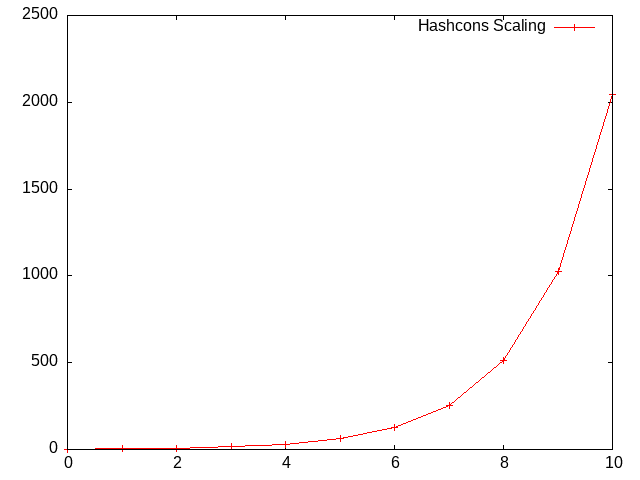
\includegraphics[width=0.6\textwidth]{figs/hashcons.png}
  \caption{Number of hashcons to add operations performed} \label{fig:hashcons}
\end{figure}
As you can see from figure \ref{fig:hashcons}, this code will perform approximately
$2^{n+1}$ hashcons operations, where n is the number of {\bf add}'s.

\subsection{Explicit Sharing and Limitations}

\cite{kiselyov:sharing} acknowledges the amount of computation with hash-consing
can get out of control, and proposes an ad-hoc solution, explicit sharing via a
custom let construct
\begin{lstlisting}{haskell}
class ExpLet repr where
  let_ :: repr a -> (repr a -> repr b) -> repr b
instance ExpLet Graph where
  let_ e f = Graph (do x <- unGraph e
                     unGraph $ f (Graph (return x)))

addChains x =
  let_ x (\x0 ->
  let_ (add x0 x0)  (\x1 ->
  let_ (add x1 x1)  (\x2 ->
   ...
  )))
\end{lstlisting}
This makes the code a bit clunky and adds an extra burden on the DSL writer, but
it prevents unnecessary hash-consing in our example. However the method has it's
limitations, suppose we want to write a DSL function that returns multiple
outputs, such as tuples or container types like lists (for example
\lstinline{haskell}{vadd :: (repr Int,repr Int) -> (repr Int,repr Int)}). %TODO
                                % need to give implementation of this function?
First of all, we need to implement different versions of the custom let construct to
correspond to the number of outputs
\begin{lstlisting}{haskell}
class ExpLet repr where
  let_ :: repr a -> (repr a -> repr b) -> repr b
  let_ 2 :: repr a -> (repr a -> (repr b,repr c)) -> (repr b,repr c)

instance ExpLet repr where
   ...
   let_2 e f = let
       g0 = Graph (do x <- unGraph e
                        let (o0,o1) = f (Graph (return x))
                        unGraph o0)
       g1 = Graph (do x <- unGraph e
                        let (o0,o1) = f (Graph (return x))
                        unGraph o1)
       in (g0,g1)
\end{lstlisting}
If need be, its possible to enumerate custom let instances for every amount of
outputs or container types we would need, we could even use template Haskell to
accomplish this. However, this custom let construct now has a new source of
redundancy in its outputs. Each output it returns will now have to individually
evaluate it's input, so a chain of DSL functions that output 2 or more values
will suffer from the same exponential scaling of hashcons.

One solution to this issue is to integrate container types such as tuples and
lists into the DSL language. However doing this will take away form the
advantages of having an embedded language, manipulating tuple values will be
cumbersome constantly requiring calls to custom implementations of {\bf
  fst}/{\bf snd} etc. And for lists you'll lose all access to built-in Haskell
list functionality.

\section{Implicit Sharing Via ByteString ASTs}

The heart of our problem is whenever we need to sequence the state of the inputs
for one of our DSL functions we want to first check if it's already been
evaluated. But how do we do that without first evaluating it to gain access to
it's unique NodeID. We need some other way to uniquely identify it.

Our proposed solution is too build an AST using byte strings along with our
DAG, but hold it outside of the State monad. We can then build our DAG using a
Trie, using the byte string AST to lookup our node identifiers instead.
% TODO reference literature on tries

\begin{lstlisting}{haskell}
data Graph a = Graph { unGraph :: State DAG NodeID
                     , stringAST :: ByteString }

data DAG = DAG { Trie (Node,NodeID)
               } deriving Show
\end{lstlisting}

The Trie essentially serves as our new BiMap, the resulting DAG contained in its
lookup values. We essentially still perform the hash-consing technique but using
the AST to perform the lookup
\begin{lstlisting}{haskell}
hashcons :: ByteString -> Node -> State DAG NodeID
hashcons sAST node = do
 DAG trie maxID <- get
 case Trie.lookup sAST trie of
   Nothing -> let maxID' = maxID+1
                  trie' = Trie.insert sAST (node,maxID+1) trie
               in do put $ DAG trie' maxID'
                     return maxID'
   Just (_,nodeID) -> return nodeID

instance Exp Graph where
  constant x = let
    node = NConstant x
    sAST = buildStringAST node []
    in Graph (hashcons sAST $ NConstant x) sAST
  variable x = let
    node = NVariable x
    sAST = buildStringAST node []
    in Graph (hashcons sAST $ NVariable x) sAST
  add e1 e2 = let
      sAST = buildStringAST (NAdd undefined undefined) [unStringAST e1,unStringAST e2]
      sT = do ns <- seqArgs [e1,e2]
              case ns of
                [n1,n2] -> hashcons sAST $ NAdd n1 n2
                _ -> error "black magic"
    in Graph sT sAST

\end{lstlisting}

The instance implementations for \lstinline{haskell}{constant} and
\lstinline{haskell}{variable} work roughly the same, the novelty of the method
is in how we handle DSL functions that take other DSL State as input like
\lstinline{haskell}{add}. First we need to construct a byte string AST from
it's input ASTs, there's a lot of ways we could go about this to attempt to
minimize memory. A naive implementation would look similar to a pretty printer.
Then we need to sequence it's inputs without evaluating the inner state if
unnecessary. We do this through the implementation of \lstinline{haskell}{seqArgs}
\begin{lstlisting}{haskell}
seqArgs :: [Graph a] -> State DAG [NodeID]
seqArgs inps =
  let
    seqArg (Graph sT sAST) =
      do DAG trie _ <- get
         case Trie.lookup sAST  trie of
           Nothing -> sT
           Just (_,nodeID) -> return nodeID
  in sequence $ map seqArg inps
\end{lstlisting}

We only evaluate the inner state \lstinline{haskell}{sT} of each argument if we
fail to look up its corresponding byte string AST in the Trie. This will prevent
redundant hashconsing without the need for explicit sharing. However this method
suffers from its own drawbacks.

\subsection{Memory Limitations}
The byte string AST being built will itself suffer from lack of sharing. We're
essentially trading extra computation for extra memory. This is often a good
tradeoff, since memory is so plentiful in modern hardware. But under the right
conditions it can become an issue

TODO include heap profiling analysis

\section{Explicit Sharing Of ByteString ASTs}
We propose another solution to this issue, taking inspiration again from the
\cite{kiselyov:sharing}, we can introduce an explicit construct for specifying
sharing. This time, the construct will substitute the current byte string for a
more compact label. For safety purposes, we need to keep track of a table of
these labels and their corresponding ASTs, to make sure we don't insert of the
same labels.
\begin{lstlisting}{haskell}
data DAG = DAG { dagTrie :: Trie (Node,NodeID)
               , dagCacheMap :: Map ByteString ByteString
               } deriving Show

data Graph a = Graph { unGraph :: State DAG NodeID
                     , stringAST :: ByteString
                     , addCache :: Maybe ByteString }

class Cacheable repr where
  cache :: ByteString -> repr ByteString -> repr ByteString
instance Cacheable Graph where
  cache s' (Graph g s _) = Graph g s' (Just s)

-- TODO better example?
test x y = let
  z = cache "z" (add x y)
  in add z z
\end{lstlisting}

The cache operation replaces the current byte string AST with a new label, and
we'll define a new operation \lstinline{haskell}{runCache} that will check if
the label already exists in the cache map before inserting it.
\begin{lstlisting}{haskell}
runCache :: ByteString -> Maybe ByteString -> Trie ByteString -> State DAG ()
runCache sAST mAddCache cacheMap = do
  case mAddCache of
    Nothing -> return ()
    Just sAST0 ->
      case Trie.lookup sAST cacheMap of
        Nothing -> let cacheMap' = Trie.insert sAST sAST0 cacheMap
                   in modify (\dag -> dag { dagCache = cacheMap' })
        Just sAST1 -> if sAST1 == sAST0
                         then return ()
                         else error $ "attempted to recache: " ++ show sAST


seqArgs :: [Graph a] -> State DAG [NodeID]
seqArgs inps =
  let
    seqArg (Graph sT sAST mCache) =
      do DAG trie cacheMap _ <- get
         runCache sAST mCache cacheMap
         ...
\end{lstlisting}
We need to make sure we don't attempt to insert the same cache label for two
different ASTs. Unfortunately, if there is a collision there's no way to escape
the State monad to prevent or modify the subtitution. The best we can do is
crash the program, or if we use a monad tansformer, we ould use
Control.Monad.Except to through an exception. Either way it's up to the DSL
writer to insure they don't reuse the same label. 

\section{Conclusion}
TODO

\subsubsection{Acknowledgements} Please place your acknowledgments at
the end of the paper, preceded by an unnumbered run-in heading (i.e.
3rd-level heading).

%
% ---- Bibliography ----
%
% BibTeX users should specify bibliography style 'splncs04'.
% References will then be sorted and formatted in the correct style.
\bibliographystyle{splncs04}
\bibliography{references}

\end{document}

% LocalWords:  DSLs unsafePerformIO Haskell's AST typeclass tagless Trie
% Local Variables:
% LaTeX-verbatim-environments-local: ("lstlisting")
% eval: (setq-local LaTeX-indent-environment-list (cons '("lstlisting" current-indentation) (default-value 'LaTeX-indent-environment-list)))
% End: